\documentclass[specialist,subf,href,colorlinks=true
%,times        % шрифт Times как основной
%,fixint=false % отключить прямые знаки интегралов
]{disser}

\usepackage[
  a4paper, mag=1000, includefoot,
  left=3cm, right=1.5cm, top=2cm, bottom=2cm, headsep=1cm, footskip=1cm
]{geometry}
\usepackage[T2A]{fontenc}
\usepackage[utf8]{inputenc}
\usepackage[english,russian]{babel}
\usepackage{placeins}
\usepackage{graphicx}
\usepackage{caption}
\usepackage{subcaption}

\ifpdf\usepackage{epstopdf}\fi

% Точка с запятой в качестве разделителя между номерами цитирований
%\setcitestyle{semicolon}

% Использовать полужирное начертание для векторов
\let\vec=\mathbf

% Включать подсекции в оглавление
\setcounter{tocdepth}{2}

\graphicspath{{fig/}}

%----------------------------------------------------------------
\begin{document}

%
% Титульный лист на русском языке
%
\thispagestyle{empty}
\begin{center}
САНКТ-ПЕТЕРБУРГСКИЙ ГОСУДАРСТВЕННЫЙ УНИВЕРСИТЕТ\\
Математико-механический факультет\\
\end{center}
%\vspace{1cm}
\begin{center}
Кафедра системного программирования\\
\end{center}
\vspace{2cm}
\begin{center}
    \Large{Классификация микроблогов с использованием Википедии} \\
\end{center}
\vspace{1cm}
\begin{center}
    \normalsize{Дипломная работа студента 545 группы} \\
    \large{Абишева Тимура Маратовича}
\end{center}
\vspace{3cm}
\noindent
\begin{center}
    \small
    \begin{tabular}{lcl}
        Научный руководитель & \dotuline{\phantom{кошерная подпись}} & к.\,ф.-м.\,н., доцент\\
        & /подпись/ & Барашев Д.В.\\
        Рецензент & \dotuline{\phantom{кошерная подпись}} & к.\,ф.-м.\,н., доцент\\
        & /подпись/&  Шалымов Д. С. \\
        ``Допустить к защите'' & \dotuline{\phantom{кошерная подпись}} & д.ф.-м.н., профессор\\
        заведующий кафедрой, & /подпись/& Терехов А.Н.\\
    \end{tabular}
\end{center}
\vspace{\fill}
\begin{center}
    \small
    Санкт-Петербург\\2012
\end{center}
\pagebreak

%%
%% Titlepage in English
%%
\thispagestyle{empty}
\begin{center}
SAINT PETERSBURG STATE UNIVERSITY\\
Mathematics & Mechanics Faculty\\
\end{center}
%\vspace{1cm}
\begin{center}
Software Engineering Chair\\
\end{center}
\vspace{2cm}
\begin{center}
    \Large{Micro blog posts classification using Wikipedia} \\
\end{center}
\begin{center}
    \large{Graduate paper} \\
    \normalsize{by} \\
    \large{Timur Abishev}
\end{center}
\vspace{3cm}
\noindent
\begin{center}
    \small
    \begin{tabular}{lcl}
        Supervisor & \dotuline{\phantom{кошерная подпись}} & PhD, Associated Professor\\
        & .................. & D. V. Barashev\\
        Reviewer & \dotuline{\phantom{кошерная подпись}} & PhD, Associated Professor\\
        & .................. & D. S. Shalymov\\
        ``Approved by'' & \dotuline{\phantom{кошерная подпись}} & Professor \\
        Head of Department, & .................. &  A. N. Terekhov\\
    \end{tabular}
\end{center}
\vspace{\fill}
\begin{center}
    \small
    Saint Petersburg\\2012
\end{center}
\pagebreak
%%% end of title pages


\tableofcontents

%\abstract
%Сервисы микроблогов, такие как, например, ``Твиттер''\footnote{https://twitter.com}, являются одной из тенденций последних лет. Эти сервисы позволяют своим пользователям публиковать сообщения различного рода, но при этом небольшой длины (в случае сервиса ``Твиттер'' --- 140 символов). Традиционные методы классификации текстов, основанные, к примеру, на модели bag-of-words \cite{wiki:bag-of-words}, для коротких текстов показывают себя несостоятельными. В данной работе описывается алгоритм классификации сообщений из ``Твиттера'' использующий веб-сервис ``Википедия''\footnote{http://en.wikipedia.org}, как источник дополнительных знаний, а также учитывающий другие сообщения автора классифицируемого сообщения. Также в данной работе происходит сравнение стандартного подхода классификации основанного на модели bag-of-words и предложенного алгоритма.
\intro

\section{Мотивация}
Сервисы микроблогов, такие как, например, ``Твиттер''\footnote{https://twitter.com}, являются одной из тенденций последних лет. Эти сервисы позволяют своим пользователям публиковать записи различного рода, но при этом небольшой длины (в случае сервиса ``Твиттер'' --- 140 символов). На момент апреля 2012 года сервисом пользовалось более 140 миллионов активных пользователей, которые публиковали до 1 миллиарда записей каждые 3 дня \cite{web:twitter-users}. 

Во время президентских выборов в США в 2008 году ``Твиттер'' использовался, в частности, для анализа позиций кандидатов \cite{Diakopoulos:2010:CDP:1753326.1753504}. Были попытки прогнозирования кассовых сборов фильмов в США с помощью ``Твиттера'' \cite{DBLP:journals/corr/abs-1003-5699}. 

Надо заметить, что активные пользователи сервиса могут получать сотни записей каждый день и далеко не всё могут прочитать сразу. Очень часто возникает желание сгруппировать полученные записи в зависимости от их тематики, чтобы  правильно расставить приоритеты чтения, что приводит нас к проблеме фильтрации записей.

С учетом вышесказанного становится понятно, что задача классификации сообщений из ``Твиттера'' является актуальной и востребованной. При наличии такого механизма классификации мы смогли бы решать разнообразные задачи, такие как: нахождение спама, разделение сообщений по разным тематикам, отделение тематических сообщений от бессодержательных. 

\section{Постановка задачи}
Целью данной дипломной работы является создание классификатора записей из микроблогов (а конкретно ``Твиттера''), который на основе обучающей выборки будет способен классифицировать записи. Для достижения данной цели были выделены следующие этапы: 
\begin{enumerate}
    \item изучение предметной области и существующих методов классификации записей из микроблогов;
    \item реализация алгоритма классификации использующего контекст записей;
    \item использование ``Википедии'' для получения неявных знаний о тексте;
    \item тестирование созданного классификатора.
\end{enumerate}

\section{Структура работы}
В главе \ref{chap:preliminaries} дается описание предметной области, вводятся понятия классификации, классификатора и кластеризации. Кроме того в данной главе рассказывается про основные метрики для оценки качества алгоритмов классификации и кластеризации, рассматриваются веб-сервисы ``Твиттер'' и ``Википедия''. В завершении главы описывается одна из простых моделей текста для задач классификации и кластеризации. 

В главе \ref{chap:bib} рассказывается о нынешнем состоянии исследований в области классификации и кластеризации микроблогов, в том числе и с учетом ``Википедии''.

В главе \ref{chap:main} рассказывается об алгоритме классификации, который предлагается в данной работе, приводится общая схема такого классификатора, его конкретные реализации с использованием стандартной модели текста, а также модели с использованием ``Википедии''.

В главе \ref{chap:experiments} приводится описание экспериментов, проделанных с разными вариантами классификаторов, и анализируется их результат.

В главе \ref{chap:tech} дается краткое описание технических решений использованных при создании классификатора.

В части ``\nameref{conclusion}'' подытоживаются полученные результаты и приводятся направления для дальнейших исследований.
\chapter{Обзор предметной области}
\label{chap:preliminaries}

\section{Используемые веб-сервисы}
\subsection{Твиттер}
``Твиттер'' является популярной социальной сетью, появившейся в 2006 году, и набравшей с тех пор более 140 миллионов активных пользователей. Основой сервиса являются публикуемые пользователями короткие сообщения, длина которых ограничена 140 символами.

Стоит отметить, что ``Твиттер'' предоставляет прикладной программный интерфейс (API) для доступа к своим данным\footnote{https://dev.twitter.com/docs/api}. Благодаря этому было создано множество библиотек для работы с данными из ``Твиттера'' на различных языках программирования.

В силу популярности сервиса, актуальности анализа его данных, а также удобства работы с ним с точки зрения создания программного обеспечения этот сервис был выбран в качестве источника данных.

\subsection{Википедия}
``Википедия'' представляет из себя свободную общедоступную энциклопедию. Главной особенностью Википедии является то, что каждый её участник может создавать, удалять и редактировать содержимое статей. Благодаря этой особенности англоязычная ``Википедия'' включает в себя порядка 4 миллионов статей (на момент мая 2012 года), а, к примеру, русскоязычная --- 800 тысяч статей\footnote{http://www.wikipedia.org/}.

Структурированность и энциклопедическая природа данных в ``Википедии'' позволяет использовать её при обработке естественных языков, к примеру, в задачах классификации и кластеризации. Данная идея не нова и существует множество исследований на данную тему. К примеру, в работе \cite{Genc:2011:DCC:2021773.2021833} сделана попытка разбить записи из ``Твиттера'' на кластеры с помощью ``Википедии''.

\section{Классификация}
\subsection{Формальное определение}
Классификацией называется задача машинного обучения с учителем. Целью классификации является разделение некоторого множества объектов на конечное, заранее известное, число классов. Для конечного подмножества объектов, называемого обучающей выборкой, класс известен заранее.

Формально, пусть $X$ --- множество описаний объектов, $Y$ --- множество номеров (или наименований) классов. Существует неизвестная ``целевая зависимость'' --- отображение $y^{*}\colon X\to Y$, значения которой известны только на объектах конечной обучающей выборки $X^m = \{(x_1,y_1),\dots,(x_m,y_m)\}$. Требуется построить алгоритм $a\colon X\to Y$, аппроксимирующий целевую зависимость\cite{wiki:ru-classification}.

Большинство алгоритмов классификации для своей работы требуют описания классифицируемых объектов в виде набора некоторых признаков или характеристик. Эти признаки бывают бинарные, номинальные, порядковые и количественные. К примеру, для текста такими признаками могут быть: ``наличие местоимений в тексте'', ``наличие сочетания 'ия' в тексте'', ``средняя длина слова меньше 5'', и т.д.

\subsection{Алгоритмы}
Существует множество подходов для реализации алгоритмов классификации. Стоит выделить такие направления, как байесовские классификаторы, нейронные сети, линейные разделители, деревья решений. Далее более подробно рассматриваются алгоритмы, используемые в данной работе.

\subsubsection{Наивный байесовский классификатор}
Наивный байесовский классификатор (Naive Bayes classifier) основан на использовании теоремы Байеса\footnote{http://ru.wikipedia.org/wiki/Теорема\_Байеса} и предполагает независимость признаков объектов.

Пусть у нас есть объект $D \in X$, имеющий признаки $\{x_1,\dots,x_n\}$, а также класс $C \in Y$. Умея оценивать $\Prob(C \vert D)\,$ мы бы могли построить классификатор по следующему правилу: $\mathrm{classify}(D) = \mathop{\mathrm{argmax}}_C \ \Prob(C \vert D)$.

Оценим $\Prob(C \vert D)$ по теореме Байеса: \begin{gather}
\Prob(C \vert D) = \Prob(C \vert x_1,\dots,x_n) = \frac{\Prob(C) \ \Prob(x_1,\dots,x_n\vert C)}{\Prob(x_1,\dots,x_n)}. \,
\end{gather}
Знаменатель является константой относительно класса $C$, так как не зависит от него, соответственно в задаче максимизации $\Prob(C \vert D)$ мы можем его игнорировать: \begin{gather}
Z = \frac{1}{\Prob(x_1,\dots,x_n)}\, \\
\Prob(C \vert D) = Z \Prob(C) \Prob(x_1,\dots,x_n\vert C).
\end{gather}

Используя предположение о независимости признаков можно получить следующий результат: \begin{gather}
\Prob(x_1,\dots,x_n\vert C) = \prod_{i=1}^n \Prob(x_i \vert C)\, \\
\Prob(C \vert D) = Z \Prob(C) \prod_{i=1}^n \Prob(x_i \vert C).
\end{gather}

Величины $\Prob(C)$ и $\Prob(x_i \vert C)$ можно оценить, подсчитав соответствующие относительные частоты в обучающей выборке. Таким образом мы получили алгоритм классификации.

\subsubsection{Метод опорных векторов}
\begin{figure}[h!]
  \centering
    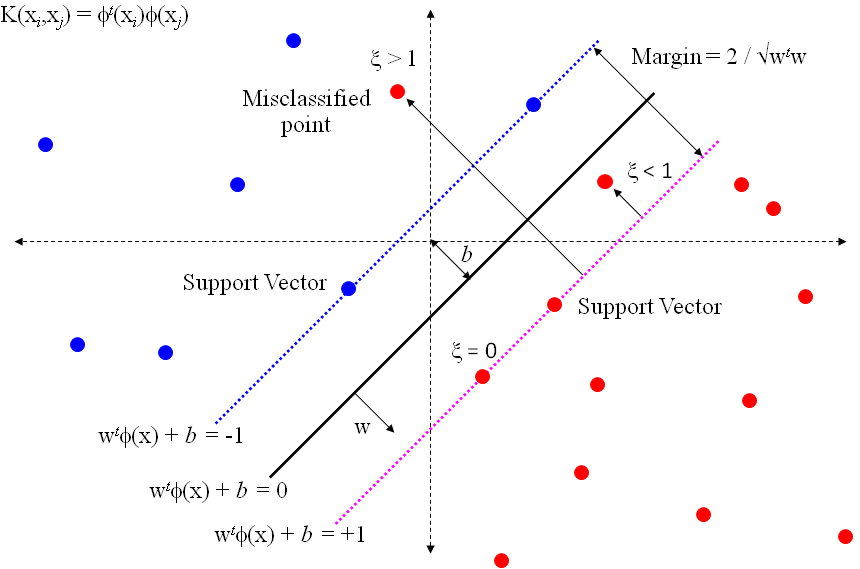
\includegraphics[width=0.7\textwidth]{svm}
    \caption{Метод опорных векторов}
\end{figure}

Данный метод (support vector machines) применим для двух классов. Основной идеей метода является попытка разделения исходной выборки с помощью гиперплоскости. В случае линейно разделимой выборки, методом ищется гиперплоскость с максимальным ``зазором'' --- суммой расстояний от плоскости до ближайших представителей обоих классов. В случае отсутствия линейной разделимости вводится понятие штрафа ($C$).
Результатом работы алгоритма является линейный классификатор задаваемый двумя параметрами: вектором $\mathbf{w}$ и константой $\mathbf{b}$. Сам алгоритм классификации задается следующим образом: $\mathrm{classify}(\mathbf{x}) = \mathrm{sign}(\mathbf{w}\cdot\mathbf{x} - b)$, где $\cdot$ --- скалярное произведение.

Стоит отметить, что в некоторых случаях применяют метод опорных векторов с каким-либо ядром. Главной идеей этого метода является замена скалярного произведения во всех операциях на какую-либо нелинейную функцию, называемую ядром. При использовании ядра, выборки, неразделимые линейным ядром, могут стать разделимыми. Однако в данной работе все случаи ядер, отличных от линейного, не рассматриваются. В частности в работе \cite{Gabrilovich:2004:TCM:1015330.1015388} сделан вывод, что для классификации текстов лучше всего подходит линейное ядро.

Для классификации более чем на два класса используется техника один-против-одного (one-against-one). Для каждой пары классов строится разделяющая гиперплоскость, в качестве итогового класса для документа выбирается тот, за который проголосовало большее число классификаторов.

\subsubsection{Деревья решений}
К данному классу алгоритмов классификации относятся алгоритмы строящие итоговый классификатор в виде дерева.
Во внутренних вершинах построенного дерева записываются условия на классифицируемый объект, в листьях --- результат классификации. Пример того, как может выглядеть дерево решения для задачи классификации людей на выживших и не выживших во время катастрофы ``Титаника''\footnote{http://ru.wikipedia.org/wiki/Титаник}, изображен на Рис. \ref{fig:titanic}. Преимуществом деревьев решений является их интерпретируемость для человека --- результат можно наглядно отобразить и проанализировать.

\begin{figure}[h!]
  \centering
    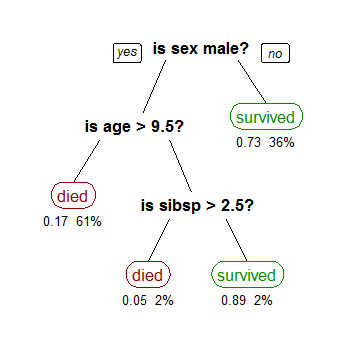
\includegraphics[width=0.7\textwidth]{titanic}
    \caption{Пример дерева принятия решений}
    \label{fig:titanic}
\end{figure}

\section{Кластеризация}
\subsection{Формальное определение}
Кластеризация --- задача машинного обучения без учителя. В данной задаче имеется множество объектов. 
Целью кластеризации является выявление групп похожих объектов, разделения объектов на классы. Главным отличием кластеризации от классификации следует считать то, что никакие характеристики групп не задаются, группы определяются полностью автоматически на основе попарной схожести объектов. 

Формально, пусть $X$ --- множество объектов, $Y$ --- множество номеров (имён, меток) кластеров. Задана функция расстояния между объектами $\rho(x,x')~$. Имеется конечная выборка объектов $X^m = \{ x_1, \dots, x_m \} \subset X$. Требуется разбить выборку на непересекающиеся подмножества, называемые ``кластерами'', так, чтобы каждый кластер состоял из объектов, близких по метрике $\rho~$, а объекты разных кластеров существенно отличались. При этом каждому объекту $x_i\in X^m$ приписывается номер кластера $y_i~$.

``Алгоритм кластеризации'' --- это функция $a\colon X\to Y$, которая любому объекту $x\in X$ ставит в соответствие номер кластера $y\in Y$. Множество $Y~$в некоторых случаях известно заранее, однако чаще ставится задача определить оптимальное число кластеров, c точки зрения того или иного ``критерия качества'' кластеризации \cite{wiki:ru-clusterization}.

Алгоритмы кластеризации, как и алгоритмы классификации, обычно имеют дело с некоторыми признаками объектов пространства $X$.

\subsection{Алгоритмы}
Входными данными для алгоритмов кластеризации выступают либо признаковые описания объектов, либо матрица попарных расстояний между объектами. Можно выделить следующие методы кластеризации: на основе графов, статистические, иерархические и на основе нейронных сетей. Стоит упомянуть, что существует задача нечеткой кластеризации, в которой, объект принадлежит кластерам с некоторой вероятностью. Далее подробней описаны алгоритмы использованные в этой работе. 

\subsubsection{Метод k-средних}
В данном алгоритме количество кластеров фиксировано величиной $k$. Задачей данного алгоритма является минимизация величины \begin{gather}
\underset{\mathbf{S}} {\operatorname{arg\,min}} \sum_{i=1}^{k} \sum_{\mathbf x_j \in S_i} \left\| \mathbf x_j - \boldsymbol\mu_i \right\|^2,
\end{gather} где $\mathbf{S}$ --- все возможные разбиения элементов $X$ на $k$ кластеров, а $\mu_i$ является центром масс кластера $S_i$. 

Задача поиска глобального минимума является NP-трудной \cite{springerlink:10.1007/s10994-009-5103-0}, однако для нее существует широко используемый алгоритм приближенного решения, находящий локальный оптимум.

Зафиксируем каким-либо образом (например случайным) $k$ первоначальных центров кластеров $m_1^{(1)}, \dots, m_k^{(1)}$. Далее алгоритм состоит из двух повторяющихся шагов:
\begin{description}
\item[Шаг присваивания] Каждому объекту из выборки $X$ сопоставляется кластер, центр которого находится к нему ближе всего: 
\begin{gather}
S_i^{(t)} = \big \{ x_p : \big \| x_p - m^{(t)}_i \big \| \le \big \| x_p - m^{(t)}_j \big \| \ \forall\ 1 \le j \le k \big\}
\end{gather}
\item[Шаг обновления] На основе объектов каждого кластера считаются новые центры: \begin{gather}
\mathbf m^{(t+1)}_i = \frac{1}{|S^{(t)}_i|} \sum_{\mathbf x_j \in S^{(t)}_i} \mathbf x_j
\end{gather}
\end{description}

Процесс заканчивается в тот момент, когда центры кластеров перестают обновляться (с какой-либо точностью). Каждый шаг алгоритма делает $O(nkt)$ действий, где $n$ --- общее количество объектов, а $t$ --- время вычисления расстояния между одной парой объектов. Данный алгоритм имеет полиномиальное количество итераций \cite{DBLP:journals/corr/abs-0904-1113}. На практике количество итераций обычно ограничивают.

\subsubsection{XMeans}
Данный алгоритм является некоторым обобщением алгоритма k-средних и использует его в своей реализации. Одним из главных отличий данного алгоритма можно назвать отсутствие требования точного количества искомых кластеров, задается лишь требуемый диапазон значений для количества кластеров. Более подробно можно прочитать в \cite{Pelleg2000}.

\section{Модель текста для классификации и кластеризации}
\label{sec:text-model}
Вышеописанные методы классификации и кластеризации применимы, если у исходных объектов есть какие-либо признаки, как это описывалось ранее. Таким образом возникает задача выделения признаков у текста.

Для решения данной задачи существует множество подходов. Опишем здесь один из самых простых. Пусть признаками в результирующем пространстве будут слова, а значениями данных признаков --- $\mathrm{tf*idf}$ данного слова относительно данного документа, где $\mathrm{tf*idf}$ определен следующим образом: \begin{gather}
\mathrm{tf}(t, d) = \frac{n_i}{\sum_k n_k} \\
\mathrm{idf}(t, D) =  \log \frac{|D|}{|d \in D : t_i \in d|} \\
\mathrm{tf*idf}(t,d,D) = \mathrm{tf}(t,d) \times \mathrm{idf}(t, D),
\end{gather} где $t$ текущее слово, $n_i$ число вхождений текущего слова в текущий документ, $\sum_k n_k$ общее количество слов в текущем документе, $d$ текущий документ, $D$ --- все документы в выборке. Величина $\mathrm{tf}$ характеризует частотность слова (терма) относительно документа, величина $\mathrm{idf}$ --- долю документов содержащих данное слово, таким образом для популярных слов величина $\mathrm{idf}$, и, соответственно $\mathrm{tf*idf}$, уменьшается.

Стоит отметить, что имеет смысл преобразовывать входной документ; к примеру, приводить слова к нормальной форме. Для данных целей служит стемминг --- процесс нахождения основы слова\footnote{http://ru.wikipedia.org/wiki/Стемминг}. Не лишено смысла применения латентно-семантического анализа\footnote{http://en.wikipedia.org/wiki/Latent\_semantic\_analysis}, для предобработки объектов. С помощью данного метода происходит выделение тематических признаков из текста. Похожий метод по выделению тематических признаков из текста с помощью метода LDA использовался в работе \cite{ramage2010characterizing}.

% другие результаты - не надо юзать ngrams
% http://know-center.tugraz.at/wp-content/uploads/2010/12/Master-Thesis-Christopher-Horn.pdf

\section{Методы оценки алгоритмов классификации}
Пусть есть построенный алгоритм классификации $a$. Для оценки качества данного алгоритма нам понадобиться дополнительная, так называемая, тестовая выборка $T$. Для данной выборки мы будем знать верные значения классов элементов. Опишем некоторые величины характеристики качества нашего алгоритма классификации: \begin{gather}
\mathrm{precision}(c) = \frac{|d \in T \colon class(d) = a(d) = c|}{|d \in T \colon a(d) = c|} \\
\mathrm{recall}(c) = \frac{|d \in T \colon class(d) = a(d) = c|}{|d \in T \colon class(d) = c|} \\
\mathrm{F}(c) = \frac{2 \mathrm{precision}(c) \mathrm{recall}(c)}{\mathrm{precision}(c) + \mathrm{recall}(c)},
\end{gather}
другими словами точность ($\mathrm{precision}$) --- это число элементов, квалифицированных правильно, по отношению к числу элементов, квалифицированных вообще, полнота ($\mathrm{recall}$) --- это число элементов, квалифицированных правильно, по отношению к общему размеру класса, а F-мера ($\mathrm{F}$) --- среднее гармоническое точности и полноты.

Недостатком этих величин является то, что они являются специфичными для классов. Введем обобщающие величины, характеризующие построенный алгоритм в целом: \begin{gather}
\mathrm{precision_{macro}} = \frac{1}{|C|} \sum_{c \in C} \mathrm{precision}(c) \\
\mathrm{recall_{macro}} = \frac{1}{|C|} \sum_{c \in C} \mathrm{recall}(c) \\
\mathrm{F_{macro}} = \frac{1}{|C|} \sum_{c \in C} \mathrm{F}(c).
\end{gather}

Данные величины можно использовать для оценки качества построенного классификатора.

\section{Методы тестирования классификаторов}
В простейшем случае нам дана как обучающая, так и тестовая выборка. Однако бывают случаи, когда тестовая выборка не дана. В этом случае разумно использовать часть обучающей выборки в качестве тестовой. 

Одним из примеров использования такого подхода является ``перекрёстная проверка'' (cross-validation). В данном методе обучающая выборка разбивается на $k$ частей, далее происходим обучение классификатора на $k-1$ части, и тестирование на оставшейся части. Процедура повторяется $k$ раз, а полученные результаты оценки качества, например, усредняются.
\chapter{Обзор литературы}
\label{chap:bib}
На текущий момент существует множество исследований связанных с вопросами классификации и кластеризации, как с использованием ``Википедии'', так и в контексте микроблогов. Существует работы классификации записей из `Твиттера` по их тональности (sentiment analysis). К примеру, в работе \cite{Go_Bhayani_Huang_2009} сообщения классифицируются по своей эмоциональной тональности; в качестве алгоритмов классификации используются метод опорных векторов, наивный байесовский метод, метод максимальной энтропии. В качестве признаков текста используются n-граммы и части речи.

Стоит отметить работу \cite{ramage2010characterizing}. В ней авторы сделали попытку кластеризовать записи из ``Твиттера'' с помощью алгоритма LDA\footnote{http://en.wikipedia.org/wiki/Latent\_Dirichlet\_allocation}. Полученные кластеры были разделены на 5 категорий: substance, status, style, social и other. 
 
Во многих работах сделаны попытки улучшения кластеризации с помощью ``Википедии''. Так в работе \cite{Genc:2011:DCC:2021773.2021833} использован сравнительно простой подход: для каждого сообщения в выборке находится наиболее релевантная статья Википедии, далее вводится метрика схожести двух статей на основе расстояния между категориями этих статей. % наверное тут еще что-то я хотел дописать

В работах \cite{Gabrilovich:2009:WSI:1622716.1622728} и \cite{Milne:2008:LLW:1458082.1458150} соответственно с помощью ``Википедии'' решаются задачи определения смысловой схожести слов, выделения ключевых слов.

Конкретно вопрос классификации записей из микроблогов рассматривается в работе \cite{Sriram:2010:STC:1835449.1835643, Horn_2010}. В первой работе рассматривается задача классификации на классы новостей, событий, мнений, предложений и личных сообщений. Во второй работе делается попытка классифицировать записи на два вида классов: на новостные, личные и от компаний, а также на мнения и факты. Также данная работа примечательна большим количеством алгоритмов участвующих в тестировании. 

\chapter{Описание алгоритма}
\label{chap:main}

\section{Общая схема}
Поставим задачу классификации. Пространством объектов для классификации будет являться пространство $Tweets$. Множеством классов --- $C$. Также у нас есть обучающая и тестовая выборки.

Имея алгоритм классификации из пространства текстов ($Texts$) в множество $C$, можно получить и алгоритм классификации для пространства $Tweets$. Назовем данный алгоритм классификации (из текстов в классы) базовым алгоритмом $\mathrm{base\_classify} \colon Texts \rightarrow C$. Как было сказано на основе этого алгоритма можно построить алгоритм классификации записей из ``Твиттера'' $\mathrm{simple\_classify} \colon Tweets \rightarrow C$.

Пусть нам дан алгоритм кластеризации сообщений из ``Твиттера'' на какое-либо пространство $Y$ $\mathrm{clusterize} \colon Tweets \rightarrow Y$. Определим новый алгоритм классификации сообщений из Твиттера:\begin{gather*} 
\mathrm{context\_classify}(tweet) = \\ \mathop{\mathrm{argmax}}_C \ | \{ neighbor \in neighbors \colon \mathrm{clusterize}(neighbor) = \mathrm{clusterize}(tweet),\\ \mathrm{simple\_classify}(neighbor) = C \}|, 
\end{gather} где $neighbors$ --- это какие-либо сообщения автора исходного сообщения для классификации $tweet$. В данной работе такими сообщениями считаются последние $n$ сообщений автора. Говоря неформальным языком, мы будем относить новую запись к тому же классу, к которому отнесли весь кластер схожих записей того же автора.

Итак, менять характеристики этого алгоритма можно меняя базовый алгоритм класификации ($\mathrm{simple\_classify}$), алгоритм кластеризации ($\mathrm{clusterize}$) и модель выделения признаков из текста, параметр $n$.

\section{Модель текста на основе ``Википедии''}
\label{sec:wiki-model}
Пример выделения признаков из текста был указан в секции \ref{sec:text-model}. В данной секции мы хотели бы привести пример альтернативного метода, основанного на Википедии. Подход описанный в данной секции частично совпадает (в разделе нахождения релевантных статей) с подходом описанным в работе \cite{MEET:MEET14504801186}. В частности, выбор констант в формулах обусловлен выводами в статье.

Хотелось бы обратить внимание на мотивацию использования ``Википедии'' для выделения признаков из текста. При использовании стандартной модели текста, к примеру, для задачи кластеризации, два текста становятся похожими только в случае использования общих слов. В случае коротких текстов (таких как в микроблогах), такие совпадения редки, и нам бы хотелось понимать, что записи содержащие слово java и слово python, являются похожими друг на друга.

Опишем алгоритм выделения признаков из текста. Данный алгоритм будет состоять из двух шагов: выделения релевантных данному тексту статей в ``Википедии'' и построению признаков по данным статьям.

\subsection{Выделение релевантных статей}
Найдем статьи на которые есть ссылки по словам участвующим в тексте. Для каждой статьи подсчитаем два значения: linking probability и overlapping rate. Пусть, к примеру, статья у нас про язык ``Haskell''\footnote{http://ru.wikipedia.org/wiki/Haskell}, а слово --- ``Haskell''. Первое значение --- отношение количества ссылок ведущих на статью к общему количеству ссылок состоящих из тех же слов (в нашем примере это отношение количества ссылок в ``Википедии'' с текстом ``Haskell'' на страницу про язык ``Haskell'' к общему количеству ссылок с текстом ``Haskell''), второе значение --- размер пересечения текста записи и текста статьи из ``Википедии'' по отношению к размеру текста сообщения с учетом стемминга. Итоговым показателем (confidence) соответствия страницы из ``Википедии'' данному тексту будет среднее арифметическое полученных linking probability и overlapping rate, таким образом $0 \leqslant \mathrm{confidence} \leqslant 1$. Далее выбирается $n$ страниц с наибольшим confidence, но большим 0.3 согласно статье \cite{MEET:MEET14504801186}. Данные статьи и являются релевантными для данного текста.

\subsection{Выделение признаков по статьям}
Для каждой страницы в ``Википедии'' определены так называемые ``категории'' --- страницы с помощью которых организуются данные в ``Википедии''. К примеру, категориями страницы соответствующей языку программирования ``Haskell''\footnote{http://ru.wikipedia.org/wiki/Haskell}, являются ``Языки программирования по алфавиту'', ``Haskell'' и ``Языки программирования семейства Haskell''. В свою очередь для категорий определены над-категории --- категории содержащие данную категорию в качестве подкатегории. Категория ``Языки программирования семейства Haskell''\footnote{ru.wikipedia.org/wiki/Категория:Языки\_программирования\_семейства\_Haskell} является под-категорией следующих категорий: ``Семейства языков программирования'', ``Функциональные языки программирования''. Основываясь на этих данных можно определить следующие множества: \begin{gather*}
\mathrm{P}(category) = \text{все над-категории категории $category$}, \\
\mathrm{C}_{0}(page) = \text{все непосредственные категории страницы $page$}, \\
\mathrm{C}_{depth}(page) = \mathrm{C}_{depth-1}(page) \bigcup \Bigl\{\bigcup_{c \in \mathrm{C}_{depth-1}(page)} \mathrm{P}(c)\Bigr\}.
\end{gather*}

Зафиксируем какое-либо значение $max\_depth$. Теперь мы можем принять категории в ``Википедии'' в качестве бинарных признаков нашего текста (есть данная категория в множестве $\mathrm{C}_{max\_depth}(page)$ или её в нем нет). В данной работе $max\_depth$ было выбрано равным 4, так как такое значение по результатам работы \cite{article:max-depth} давало наилучший результат.

\chapter{Эксперименты}
\label{chap:experiments}

\section{Тестовая выборка}
Для тестирования разработанной схемы для создания классификаторов необходимо создать тестовую выборку. Данная глава описывает четыре набора данных использованных для тестирования.

\subsection{Тематические классы}
Данный тестовый набор состоит из следующих классов:
\begin{itemize}
\item Физика
\item Химия
\item Биология
\item Математика
\item Программирование
\end{itemize}

Для каждого из классов были выбраны несколько пользователей ``Твиттера'', которые пишут на данную тему. Они перечислены в Таблице \ref{table:thematic}. Далее для каждого из пользователей в выборку вошли случайные 100 записей из последних 2000.

В качестве способа тестирования было выбрано два варианта: перекрёстная проверка с разделением на 4 части и тестовая выборка составленная из записей пользователей отличных от тех, что использовались в обучающей выборке.

\subsection{Целевые классы}

Данный тестовый набор частично взят из работы \cite{Horn_2010}. Он состоит из классов:
\begin{itemize}
\item Новостных сообщений
\item Персональных сообщений
\item Сообщений из официальных ``Твиттер'' аккаунтов компаний
\end{itemize}

Как и предыдущий, этот тестовый набор составлялся на основе пользователей ``Твиттера''. В Таблице \ref{table:unc} перечислены пользователи с классами к которым они были отнесены.

В качестве способа тестирования была выбрана перекрёстная проверка с разделением на 4 части и тестовая выборка составленная из записей пользователей отличных от тех, что использовались в обучающей выборке.

\section{Алгоритмы}
\subsection{Простая классификация}
К данной секции относятся следующие классифицирующие алгоритмы: \begin{itemize}
\item наивный байесовский,
\item метод опорных векторов,
\item метод J48 для построения деревьев принятия решений.
\end{itemize}

Все эти алгоритмы на вход принимают объекты из пространства признаков, так что использовалось два метода для выделения признаков из текста: \begin{itemize}
\item простая модель, описанная в секции \ref{sec:text-model};
\item модель на основе ``Википедии'' (далее --- энциклопедическая), описанная в секции \ref{sec:wiki-model}.
\end{itemize}

В общем получается 6 вариантов алгоритма.

\subsection{Классификация с учетом контекста}
В данной секции использовался предложенный в работе алгоритм классификации. В качестве базового алгоритма были использованы те же алгоритмы, что и в предыдущей секции, аналогично для алгоритма выделения признаков из текста. В качестве кластеризующих были использованы следующие алгоритмы: \begin{itemize}
\item k-means на 20 кластеров,
\item k-means на 100 кластеров,
\item xmeans с параметрами от 20 до 100 кластеров.
\end{itemize}

Во всех алгоритмах в качестве метрики для расстояния использовалась евклидова метрика\footnote{http://ru.wikipedia.org/wiki/Евклидова\_метрика}. Количество последних сообщений для кластеризации --- 2000.

В общем получается 18 вариантов алгоритма.

\section{Результаты экспериментов}

% Тематические классы: тестовая выборка
\begin{figure}[h!]
  \centering
    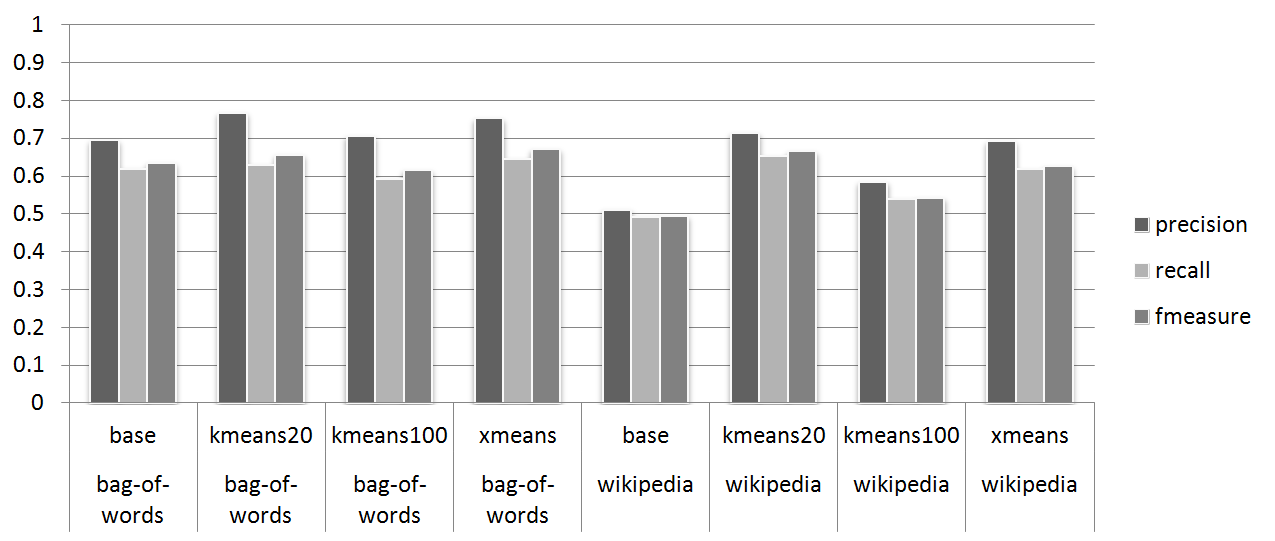
\includegraphics[width=\textwidth]{thematic/test/naive}
    \caption{Тематические классы: тестовая выборка; наивный байесовский классификатор}
    \label{fig:thematic-test-naive}
\end{figure}

\begin{figure}[h!]
  \centering
    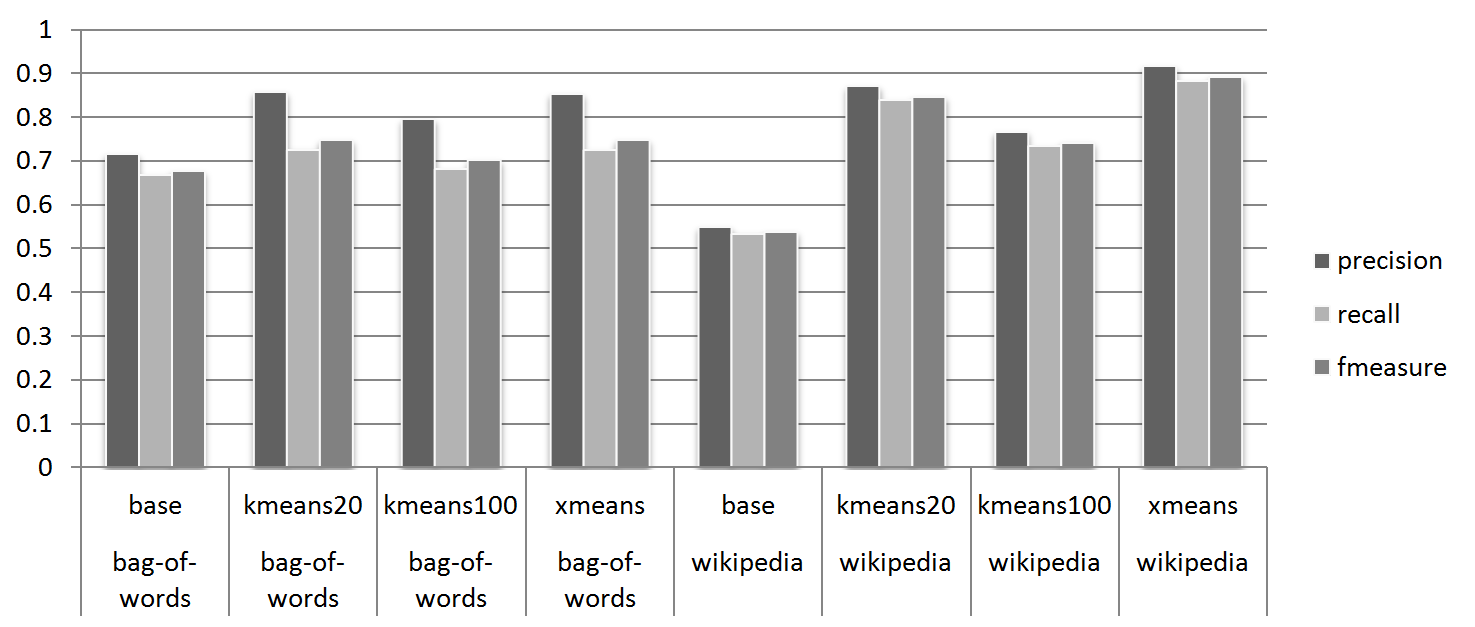
\includegraphics[width=\textwidth]{thematic/test/svm}
    \caption{Тематические классы: тестовая выборка; метод опорных векторов}
    \label{fig:thematic-test-svm}
\end{figure}

\begin{figure}[h!]
  \centering
    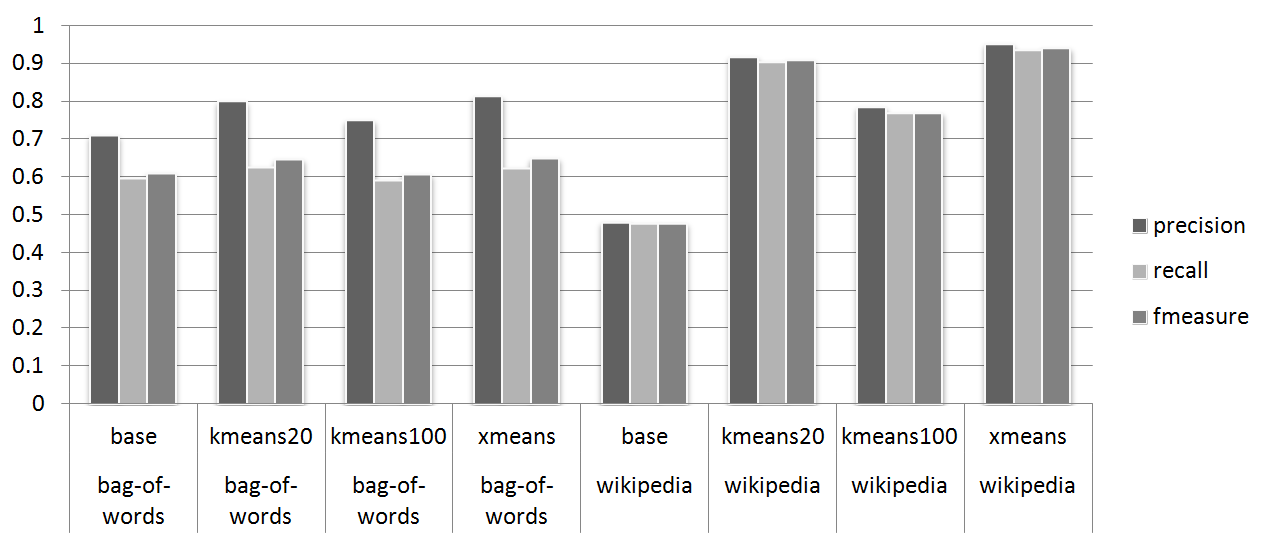
\includegraphics[width=\textwidth]{thematic/test/j48}
    \caption{Тематические классы: тестовая выборка; алгоритм построения деревьев решений J48}
    \label{fig:thematic-test-j48}
\end{figure}

% Тематические классы: перекрёстная проверка
\begin{figure}[h!]
  \centering
    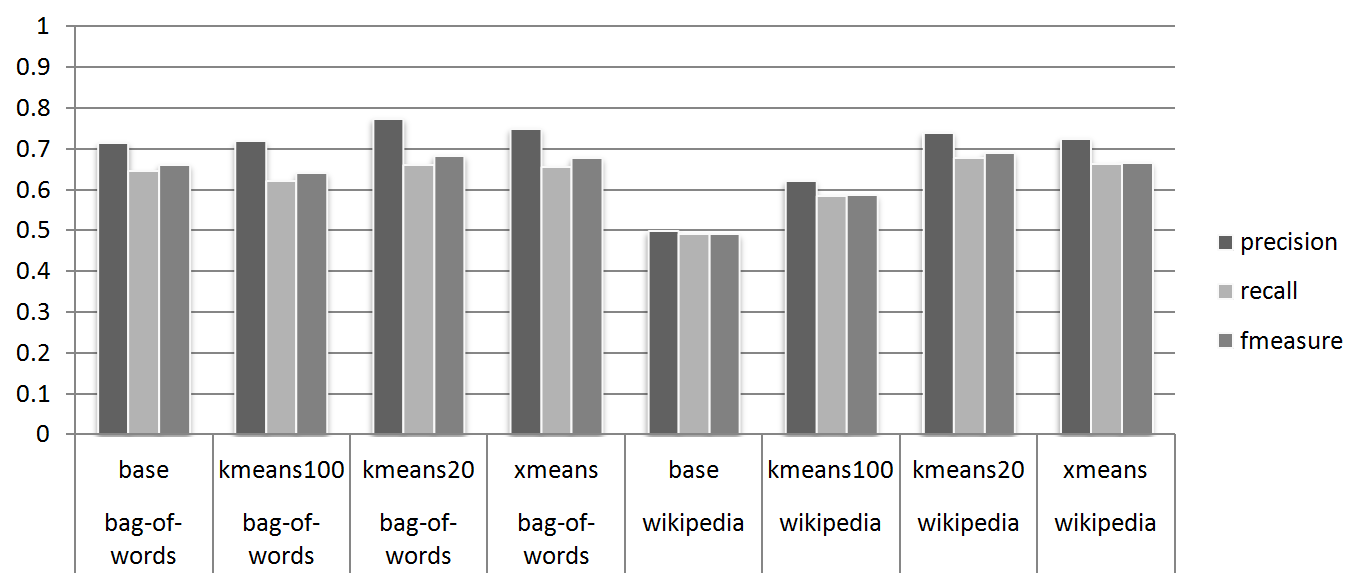
\includegraphics[width=\textwidth]{thematic/cross/naive}
    \caption{Тематические классы: перекрёстная проверка; наивный байесовский классификатор}
    \label{fig:thematic-cross-naive}
\end{figure}

\begin{figure}[h!]
  \centering
    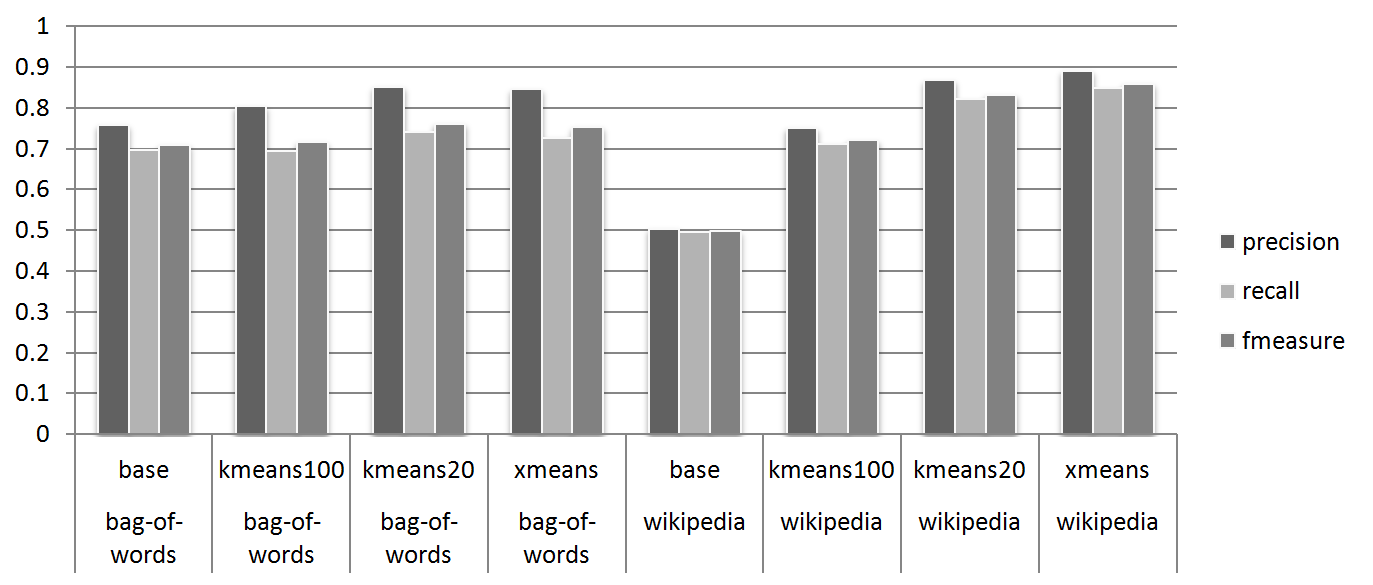
\includegraphics[width=\textwidth]{thematic/cross/svm}
    \caption{Тематические классы: перекрёстная проверка; метод опорных векторов}
    \label{fig:thematic-cross-svm}
\end{figure}

\begin{figure}[h!]
  \centering
    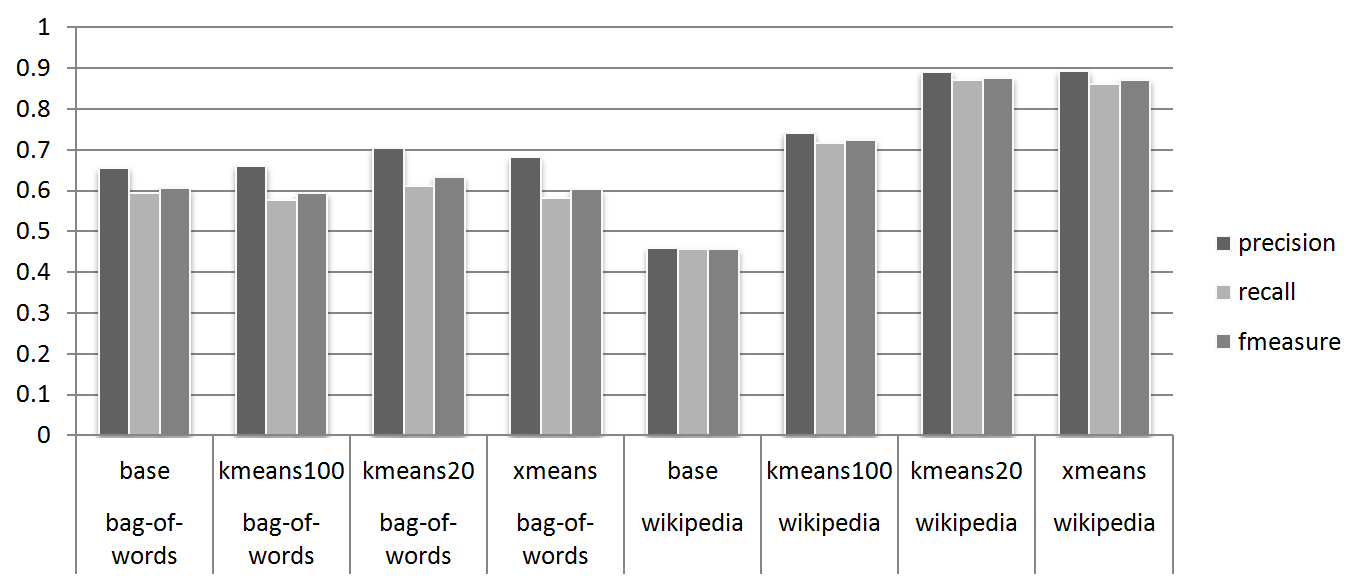
\includegraphics[width=\textwidth]{thematic/cross/j48}
    \caption{Тематические классы: перекрёстная проверка; алгоритм построения деревьев решений J48}
    \label{fig:thematic-cross-j48}
\end{figure}

% Целевые классы: тестовая выборка
\begin{figure}[h!]
  \centering
    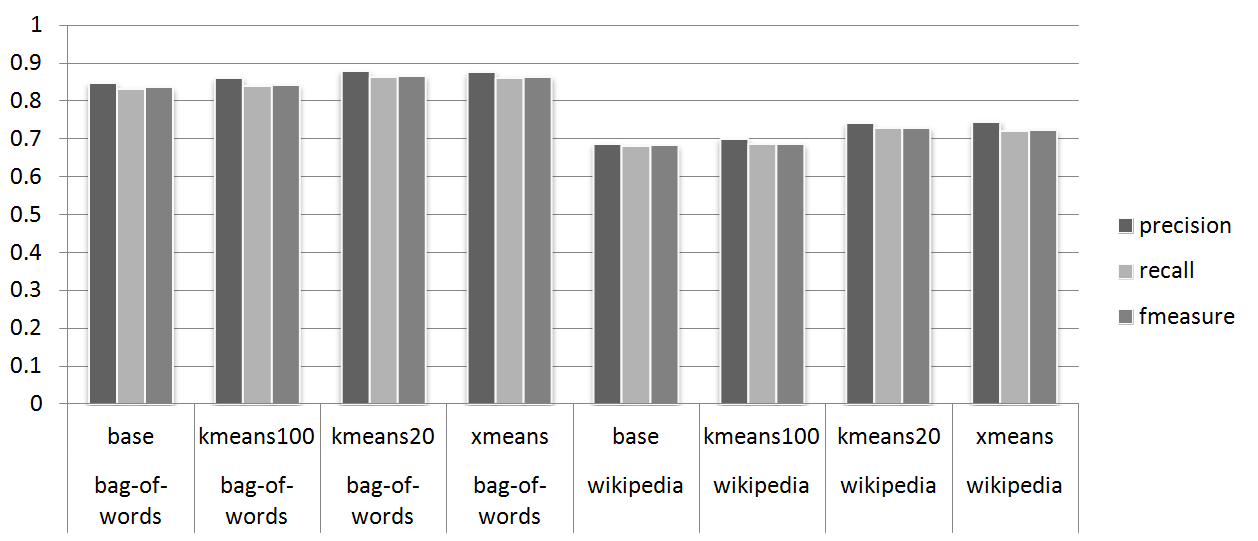
\includegraphics[width=\textwidth]{usernewscompany/test/naive}
    \caption{Целевые классы: тестовая выборка; наивный байесовский классификатор}
    \label{fig:usernewscompany-test-naive}
\end{figure}

\begin{figure}[h!]
  \centering
    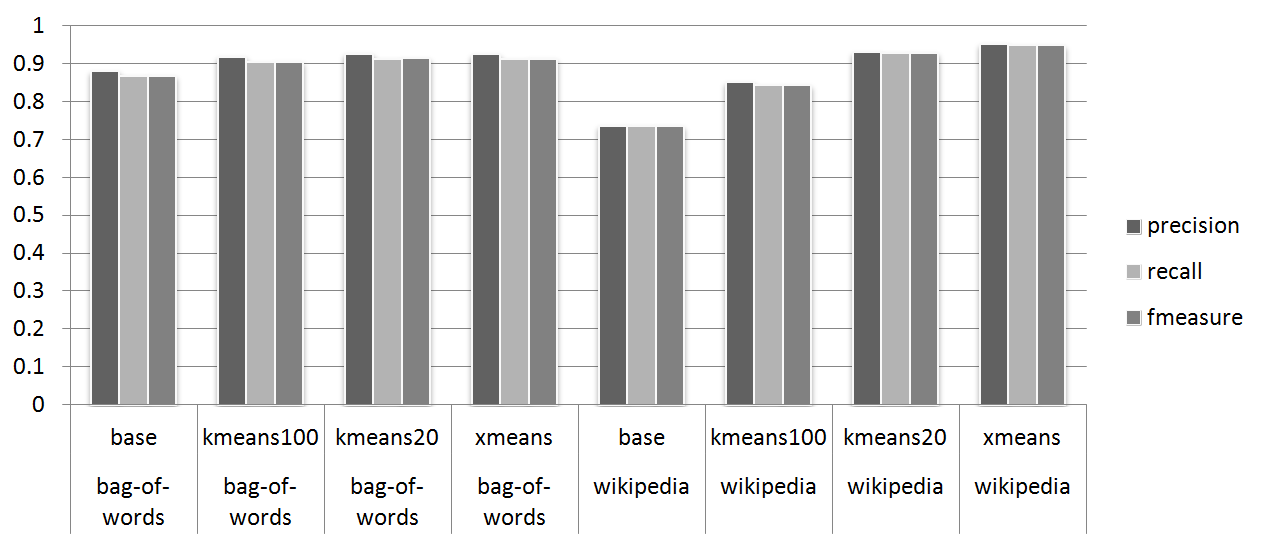
\includegraphics[width=\textwidth]{usernewscompany/test/svm}
    \caption{Целевые классы: тестовая выборка; метод опорных векторов}
    \label{fig:usernewscompany-test-svm}
\end{figure}

\begin{figure}[h!]
  \centering
    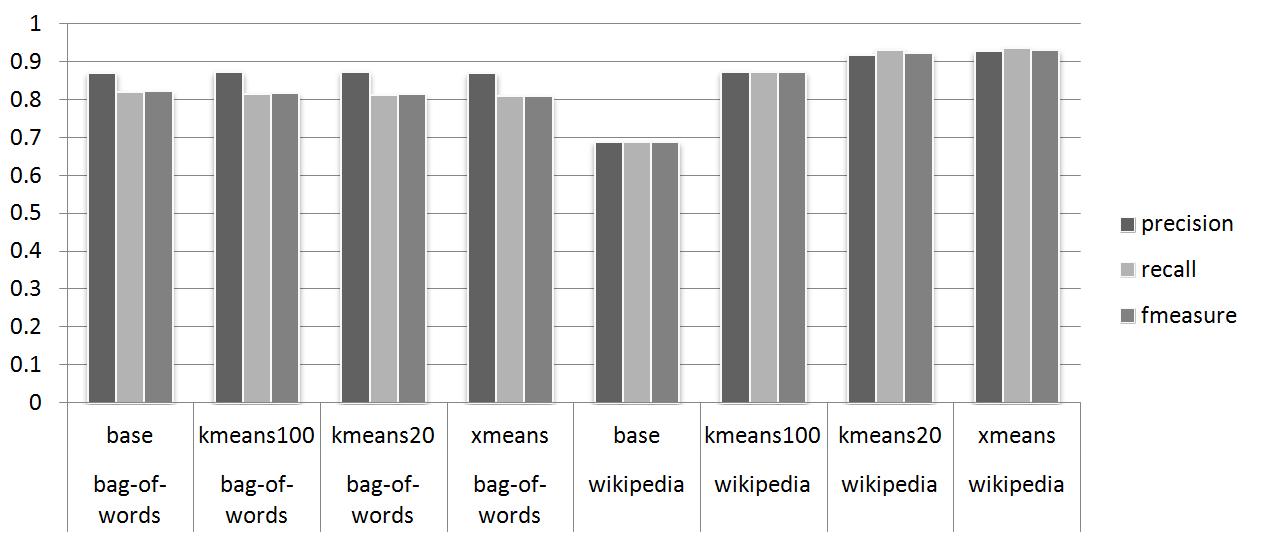
\includegraphics[width=\textwidth]{usernewscompany/test/j48}
    \caption{Целевые классы: тестовая выборка; алгоритм построения деревьев решений J48}
    \label{fig:usernewscompany-test-j48}
\end{figure}

% Целевые классы: перекрёстная проверка
\begin{figure}[h!]
  \centering
    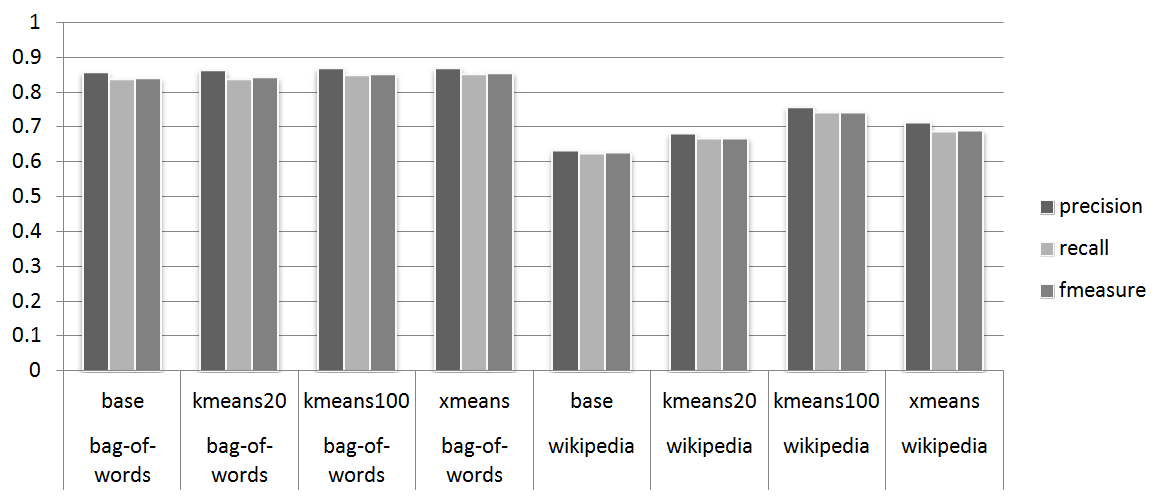
\includegraphics[width=\textwidth]{usernewscompany/cross/naive}
    \caption{Целевые классы: перекрёстная проверка; наивный байесовский классификатор}
    \label{fig:usernewscompany-cross-naive}
\end{figure}

\begin{figure}[h!]
  \centering
    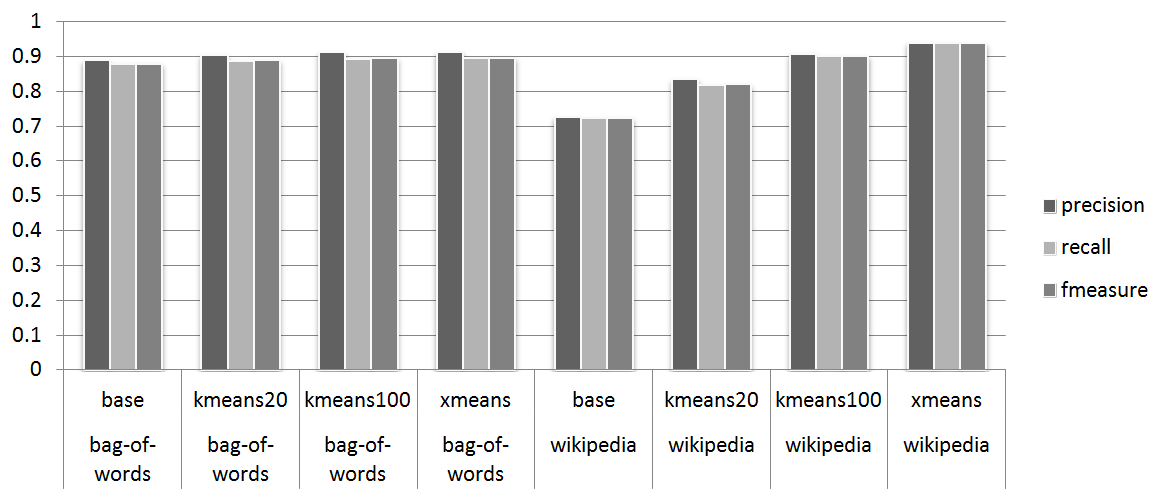
\includegraphics[width=\textwidth]{usernewscompany/cross/svm}
    \caption{Целевые классы: перекрёстная проверка; метод опорных векторов}
    \label{fig:usernewscompany-cross-svm}
\end{figure}

\begin{figure}[h!]
  \centering
    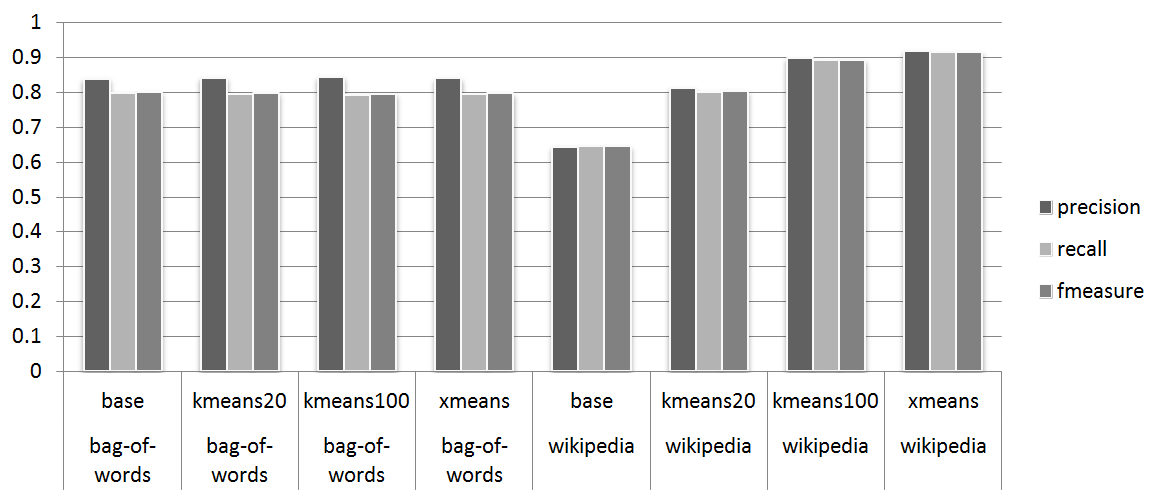
\includegraphics[width=\textwidth]{usernewscompany/cross/j48}
    \caption{Целевые классы: перекрёстная проверка; алгоритм построения деревьев решений J48}
    \label{fig:usernewscompany-cross-j48}
\end{figure}

Для начала хотелось бы отметить, что метод опорных векторов продемонстрировал наилучшие результаты на наших тестовых данных (рисунки  \ref{fig:thematic-test-svm}, \ref{fig:thematic-cross-svm}, \ref{fig:usernewscompany-test-svm}, \ref{fig:usernewscompany-cross-svm}). Кроме того, метод опорных векторов больше всех выигрывает от использования контекста в классификаторе (это лучше заметно на рисунках соответствующих тематической тестовой выборке: \ref{fig:thematic-test-svm} и \ref{fig:thematic-cross-svm}). Меньше всех выигрывает, а иногда даже проигрывает от использования контекста наивный байесовский классификатор. Также можно видеть не самый успешный результат алгоритма J48 в случае использования простой модели текста (Рис. \ref{fig:thematic-cross-j48}).

При использовании энциклопедической модели теста, к сожалению, результат простых классификаторов значительно ухудшился. Этот результат показывает, что данный аспект, по всей видимости, нуждается в улучшении. Однако стоит отметить, что использование контекста в случае энциклопедической модели позволяет получить значительное (порядка 20\% на Рис. \ref{fig:thematic-test-svm}) улучшение показателей классификатора. Связка признаков из ``Википедии'', использования контекста и метода опорных векторов продемонстрировала наилучший результат в данной работе.

Стоит отметить, что при использовании контекста, улучшение на первом наборе данных было больше чем на втором. Это выглядит разумным в свете того, что кластеризация более вероятно объединяет сообщения похожие тематически, чем по каким-либо других критериям. 

Из алгоритмов кластеризации наиболее предпочтительно выглядит XMeans. Именно этот алгоритм рекомендуется использовать при использовании контекстной классификации.
\chapter{Технические решения}
\label{chap:tech}
Для реализации всех алгоритмов классификации и кластеризации используется открытая библиотека Weka\footnote{http://www.cs.waikato.ac.nz/ml/weka/}. Основным языком реализации была выбрана Java\footnote{http://java.com} в силу своей распространенности и мультиплатформенности. Для работы с ``Википедией'' применяется библиотека wikixmlj\footnote{http://code.google.com/p/wikixmlj/}. Для работы с ``Твиттером'' применяется библиотека twitter4j\footnote{http://twitter4j.org/en/index.html}.

Итоговое решение можно разделить на следующие части: часть для работы с ``Твиттеров'', часть для работы с ``Википедией'', часть содержащая алгоритм классификации и тестирования. Для реализации контекстного классификатора был создан класс ContextClassifier, реализующий класс Classifier библиотеки Weka. В качестве параметров данного классификатора выступают фабрика\footnote{http://ru.wikipedia.org/wiki/Абстрактная\_фабрика\_(шаблон_проектирования)} для создания базовых классификаторов, фабрика алгоритмов кластеризации, модель выделения признаков из текста. Модель выделения признаков из текста реализована в виде наследника класса Filter библиотеки Weka.   

Диаграмму классов алгоритмов классификации можно увидеть на Рис. \ref{fig:uml-classifiers}, кластеризации на Рис. \ref{fig:uml-clusterers}, выделения признаков из текста на Рис. \ref{fig:uml-models}.

% http://yuml.me/diagram/plain/class/[Classifier|buildClassifier(data);classifyInstance(instance)]^-[ContextClassifier|classifier;clusterer;wordModel],[Classifier|buildClassifier(data);classifyInstance(instance)]^-[NaiveBayes],[Classifier|buildClassifier(data);classifyInstance(instance)]^-[MISVM],[Classifier|buildClassifier(data);classifyInstance(instance)]^-[J48]

\begin{figure}[h!]
  \centering
    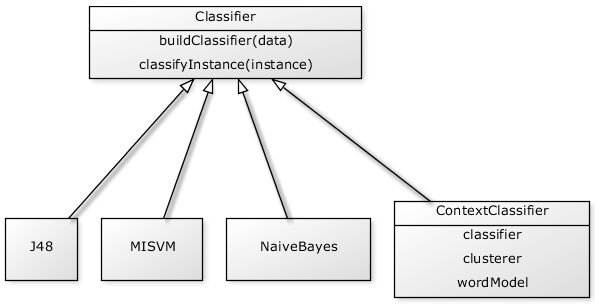
\includegraphics[width=0.7\textwidth]{uml/classifiers}
    \caption{Классы для классификации}
    \label{fig:uml-classifiers}
\end{figure}

% http://yuml.me/diagram/plain/class/[Filter]^-[MapFilter|map(data)],[MapFilter|map(data)]^-[WikiTextModel],[Filter]^-[StringToWordVector]

\begin{figure}[h!]
  \centering
    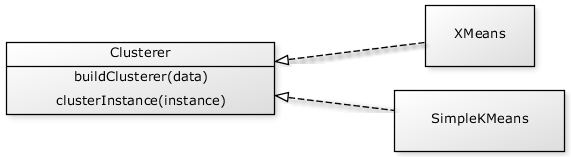
\includegraphics[width=0.7\textwidth]{uml/clusterers}
    \caption{Классы для кластеризации}
    \label{fig:uml-clusterers}
\end{figure}

% http://yuml.me/diagram/plain/class/[Clusterer|buildClusterer(data);clusterInstance(instance)]^-.-[SimpleKMeans],[Clusterer|buildClusterer(data);clusterInstance(instance)]^-.-[XMeans]

\begin{figure}[h!]
  \centering
    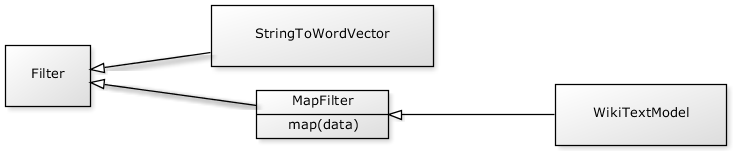
\includegraphics[width=0.7\textwidth]{uml/models}
    \caption{Классы для выделения признаков из текста}
    \label{fig:uml-models}
\end{figure}

\conclusion
\label{conclusion}

\section{Результаты}
В результате данной работы была изучена предметная область, придуман и реализован алгоритм классификации записей из микроблогов. Реализованный алгоритм имеет несколько особенностей: он использует контекст записей, а также ``Википедию'', как источник дополнительных знаний.

Данный алгоритм был протестирован на нескольких вариантов тестовых данных. В некоторых случаях алгоритм показал хорошие результаты и продемонстрировал существенное улучшение в сравнении с простым подходом для классификации записей.

\section{Дальнейшая работа}
Большим пространством для дальнейших исследований представляется улучшение алгоритма выделения признаков из текста с использованием ``Википедии''. Стоит отметить, что возможно стоит попробовать другие алгоритмы кластеризации, например, k-medoids\footnote{http://en.wikipedia.org/wiki/K-medoids}, как не требующий представления документов в пространстве признаков (данный алгоритм требует только расстояние между элементами выборки). Имеет смысл попробовать применить латентно-семантический анализ, для предобработки признаковых представлений объектов, для улучшения результата в задачах классификации и кластеризации. Также стоит подготовить б\'oльшие обучающие и тестовые выборки для более полного тестирования полученных алгоритмов. 

Кроме того разработанный алгоритм работает очень долго, что сильно осложняет его тестирование. Было проведено профилирование, в ходе которого было обнаружено, что наибольшую часть времени занимает процесс построения кластеров и непосредственно классификации. В частности, проблема заключается в том, что код библиотеки Weka является однопоточным. Можно, к примеру, распараллелить алгоритмы кластеризации, контекстной классификации, а также тестирование методом перекрёстной проверки. 

\appendix
\chapter{Пользователи Твиттера, выбранные для тестовых данных}
\section{Для тематических классов}

\label{table:thematic}
\begin{tabular}[t]{|c|l|}
\hline
Пользователь & Класс \\
\hline
carnage4life & programming \\
\hline
stevenf & programming \\
\hline
jasonfried & programming \\
\hline
codinghorror & programming \\
\hline
PhysicsNews & physics \\
\hline
materion & physics \\
\hline
CERN & physics \\
\hline
Math\_Bits & math \\
\hline
mathguide & math \\
\hline
AlgebraFact & math \\
\hline
ChemistryBooks & chemistry \\
\hline
NatureChemistry & chemistry \\
\hline
ChemistryWorld & chemistry \\
\hline
tlemberger & biology \\
\hline
BioscienceNews & biology \\
\hline
CHoytPhD & biology \\
\hline
pzmyers & biology \\
\hline
\end{tabular}

\section{Для разделения на персональный/новостной/принадлежит компании}

\label{table:unc}
\begin{tabular}[t]{|c|l|}
\hline
Пользователь & Класс \\
\hline
ladygaga & user \\
\hline
johnbreslin & user \\
\hline
PerezHilton & user \\
\hline
tony & user \\
\hline
davejmatthews & user \\
\hline
saturdaystar & news \\
\hline
HurriyetDaily & news \\
\hline
MoscowTimes & news \\
\hline
latimes & news \\
\hline
TelegraphMG & news \\
\hline
arielgabriel & company \\
\hline
xemmy & company \\
\hline
myeverydaymoney & company \\
\hline
dealnaydotcom & company \\
\hline
compudah & company \\
\hline
\end{tabular}


\bibliography{thesis}
\bibliographystyle{gost705}
\end{document}

